% import packages
\documentclass[8pt,table=xcolor,usenames,dvipsnames]{beamer}
\usepackage[utf8]{inputenc}
\usepackage{colortbl}
\usepackage{ragged2e}
\usepackage{booktabs}
\usepackage{threeparttable}
\usepackage{pifont}
\usepackage{graphicx}
\usepackage{hhline}
\usepackage{amsmath}
\usepackage{amssymb}
\usepackage{amsthm}
\usepackage{tikz}
\usepackage{bm}
\usepackage{etoolbox}
\usepackage[export]{adjustbox}
\usepackage[justification=centering]{caption}
\usepackage[backend=bibtex,style=authoryear,maxcitenames=2,natbib=true,maxbibnames=99]{biblatex}

% patch circles for framebreaks
% source: https://tex.stackexchange.com/a/132312
\makeatletter
\patchcmd{\slideentry}{\ifnum#2>0}{\ifnum2>0}{}{}
\patchcmd{\slideentry}{\c@subsectionslide}{\c@framenumber}{}{}
\patchcmd{\beamer@writeslidentry}{\c@subsectionslide}{\c@framenumber}{}{}
\makeatother

% set beamer parameters
\usetheme{Frankfurt}
\usecolortheme{default}
\setbeamerfont{footnote}{size=\Tiny}
\setbeamertemplate{page number in head/foot}{}
\setbeamertemplate{bibliography item}{}
\setbeamertemplate{caption}[numbered]
\setbeamercovered{transparent}
\setbeamerfont{institute}{size=\small}
\addtobeamertemplate{navigation symbols}{}{%
  \usebeamerfont{footline}%
  \usebeamercolor[fg]{footline}%
  \hspace{2em}%
  \raisebox{1.7pt}[0pt][0pt]{\insertframenumber/\inserttotalframenumber}
}
\setbeamertemplate{enumerate items}[square]
\setbeamertemplate{section in toc}[square]
\setbeamertemplate{theorems}[numbered]

% special command to uncover graphics
% source: https://tex.stackexchange.com/a/415335
\newcommand<>{\uncovergraphics}[2][{}]{
  % Taken from: <https://tex.stackexchange.com/a/354033/95423>
  \begin{tikzpicture}
    \node[anchor=south west,inner sep=0] (B) at (4,0)
    {\includegraphics[#1]{#2}}; \alt#3{}{%
      \fill [draw=none, fill=white, fill opacity=0.7] (B.north west) -- (B.north
      east) -- (B.south east) -- (B.south west) -- (B.north west) -- cycle; }
  \end{tikzpicture}
}

% set caption parameters
\DeclareCaptionFormat{myformat}{\fontsize{6}{6}\selectfont#1#2#3}
\captionsetup{format=myformat}
\captionsetup[figure]{labelfont={bf},name={Figure}}
\captionsetup[table]{labelfont={bf},name={Table}}

% set bibliography parameters
\renewcommand\refname{Bibliography}
\addbibresource{../bibtex.bib}
\setlength\bibitemsep{1.5\itemsep}
\let\oldcitep=\citep
\renewcommand\citep[1]{{\textcolor{blue}{\oldcitep{#1}}}}
\let\oldcitet=\citet
\renewcommand\citet[1]{{\textcolor{blue}{\oldcitet{#1}}}}

% miscellaneous settings
\settowidth{\leftmargini}{\usebeamertemplate{itemize item}}
\addtolength{\leftmargini}{\labelsep}
\renewcommand{\arraystretch}{1.3}
\graphicspath{{../visuals/}}
\newcolumntype{L}[1]{>{\RaggedRight\hspace{0pt}}p{#1}}

% set admin details
\title{Language detection using character n-gram profiles}
\subtitle{Inspiration from Cavnar and Trenkle (1994)}
\author{Atreya Shankar \\ Applying for: Scientific Researcher in NLP}
\date{July 6, 2021}

% start presentation
\begin{document}
\begin{frame}
  \maketitle
\end{frame}

\begin{frame}
  \frametitle{Overview}
  \tableofcontents
\end{frame}

\section{Introduction}

\begin{frame}
  \frametitle{Motivation}
  \begin{figure}
    \centering
    \begin{tikzpicture}
      \setlength{\fboxsep}{1pt}
      \node[anchor=south west,inner sep=0] at (0,0) {
        \fbox{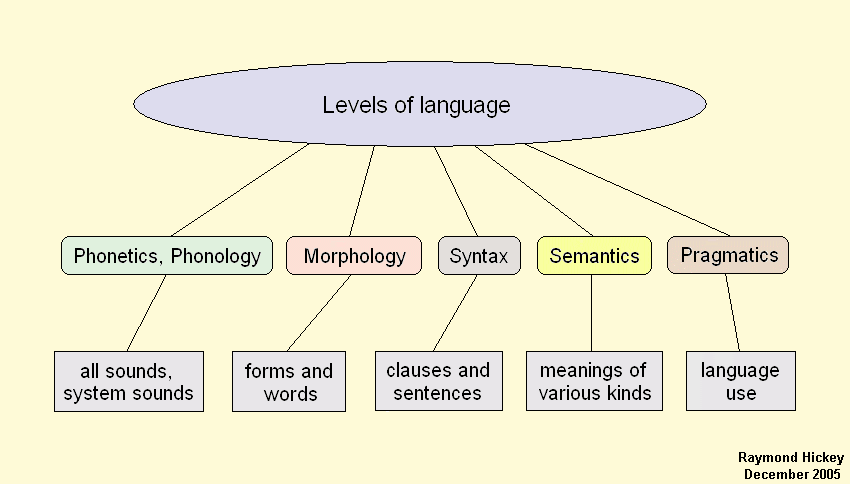
\includegraphics[width=9cm]{levels.png}}};
      \draw<2->[red, thick] (3,2.2) rectangle (4.6,2.75);
    \end{tikzpicture}
    \caption{Levels/structures of languages; figure taken from \citet{hickey2005levels}}
  \end{figure}
  \uncover<3>{\begin{itemize}
      \item Morphological profiling probably has lower data and compute requirements
      \item Makes sense given no external libraries are allowed
    \end{itemize}}
\end{frame}

\section{Methodology}

\begin{frame}
  \frametitle{Methodology}
  \begin{columns}[T]
    \begin{column}{.40\textwidth}
      \begin{itemize}          
        \setlength\itemsep{1.5em}
        \uncover<1>{
          \item Character n-gram profiling technique from \citet{cavnar1994n}
          \item WiLI-2018 data set for 235 languages with 235,000 paragraphs
          \citep{thoma2018wili}}
        \uncover<2>{
          \item \textbf{Similarities:} Data is lower-cased and punctuation/special-tokens are removed
          \item \textbf{Differences:} Use vector-based difference norm instead of
          out-of-place distance 
          \item \textbf{Two hyperparameters:} character n-gram length and ranked n-gram cutoff
        }
      \end{itemize}
    \end{column}
    \hfill
    \begin{column}{.60\textwidth}
      \captionsetup{width=5.5cm} 
      \centering \uncovergraphics<1>[width=3cm,valign=t]{title.pdf}
      \uncover<1>{\captionof{figure}{Excerpt from \citet{cavnar1994n}}}
      \label{fig:title}
      \uncovergraphics<2>[height=4.5cm,valign=t]{dataflow.pdf}
      \uncover<2>{\captionof{figure}{Flowchart from \citet{cavnar1994n}}}
      \label{fig:dataflow}
    \end{column}
  \end{columns}
\end{frame}

\section{Results}

\begin{frame}
  \frametitle{Results}
  \uncover<1>{\begin{table}[t!]
      \centering
      \begin{tabular}{L{0.1\linewidth} L{0.1\linewidth} L{0.15\linewidth} L{0.15\linewidth} L{0.15\linewidth}}
        \toprule
        N-gram length & N-gram \qquad cutoff & Weighted Test F$_1$ & Best \qquad Language & Worst \qquad Language \\
        \midrule
        2 & 100 & 0.865 & Navajo & Konkani \\ 
        2 & 300 & 0.893 & Navajo & Pampanga \\
        3 & 100 & 0.859 & Dhivehi & Chavacano \\
        \textbf{3} & \textbf{300} & \textbf{0.898} & Navajo & Chavacano \\
        \bottomrule
      \end{tabular}
      \caption{Tabular summary of model performances; MLP from
        \citet{thoma2018wili} achieved an accuracy of 0.883}
      \label{tab:results}
    \end{table}}

  \uncover<2>{\begin{table}[t!]
      \centering
      \begin{tabular}{L{0.15\linewidth} L{0.1\linewidth} L{0.1\linewidth} L{0.1\linewidth} L{0.1\linewidth} L{0.1\linewidth}}
        \toprule
        Language & N$_1$ & N$_2$ & N$_3$ & N$_4$ & N$_5$ \\
        \midrule
        English & \textit{the} & \textit{and} & \textit{ing} & \textit{ion} & \textit{ent} \\
        Deutsch & \textit{der} & \textit{sch} & \textit{die} & \textit{ein} & \textit{che} \\
        Italiano & \textit{del} & \textit{ell} & \textit{ent} & \textit{ion} & \textit{lla} \\
        \bottomrule
      \end{tabular}
      \caption{Tabular summary of top five character trigrams with highest
        relative frequency per language}
      \label{tab:analysis}
    \end{table}}
\end{frame}

\section{Discussion}

\begin{frame}
  \frametitle{Discussion}
  \uncover<1>{\begin{table}[t!]
      \centering
      \begin{tabular}{L{0.2\linewidth} L{0.25\linewidth} L{0.25\linewidth}}
        \toprule
        Gold language & Utterance & Predicted language \\
        \midrule
        English & \textit{What is this?} & Cantonese \\
        Deutsch & \textit{Was ist das?} & Chavacano \\
        Italiano & \textit{Cos'è questo?} & Asturian \\
        \bottomrule
      \end{tabular}
      \caption{Examples of erroneous language detection for short phrases}
      \label{tab:short}
    \end{table}

    Plenty of failing cases: \setlength{\leftmargini}{0.5cm}
    \begin{itemize}      
      \setlength\itemsep{0.5em}
      \item Short phrases where language profile cannot converge
      \item Slang, colloquial or borrowed words
      \item Transliteration from non-Latin to Latin script
    \end{itemize}}

  \vspace{15pt}
  
  \uncover<2>{
    Plenty of workarounds: \setlength{\leftmargini}{0.5cm}
    \begin{itemize}      
      \setlength\itemsep{0.5em}
      \item Word-level language identification with large-enough vocabulary
      \item Complex modeling over sequential subwords, for example using neural
      networks; such as in \citet{DBLP:journals/corr/abs-1708-04811}
    \end{itemize}
  }
\end{frame}

\section{Conclusions}

\begin{frame}
  \frametitle{Conclusions}
  \begin{itemize}    
    \setlength\itemsep{1.5em}
    \uncover<1>{\item Portable and lightweight character n-gram profiling technique from
      \citet{cavnar1994n}
      \item Trained and tested on WiLI-2018 \citep{thoma2018wili}
      \item Best character trigram model achieved \textbf{89.8\%} weighted F$_1$ test score}
    \uncover<2>{\item Works well for medium-long length documents, likely robust to
      previously unseen words and spelling errors
      \item Known limitations on short length documents} 
  \end{itemize}
\end{frame}

\section*{Bibliography}

\begin{frame}[allowframebreaks]
  \frametitle{Bibliography}
  \nocite{*}
  \printbibliography[title = {Bibliography}, heading=none]
\end{frame}

\end{document}

% LocalWords:  Cavnar Trenkle Atreya Shankar NLP WiLI hyperparameters Konkani
% LocalWords:  Pampanga Dhivehi Chavacano MLP ing ent Deutsch der ein che del
% LocalWords:  Italiano lla trigrams ist das Cos'è questo Asturian subwords
% LocalWords:  trigram
